\documentclass[tikz]{standalone}

\begin{document}

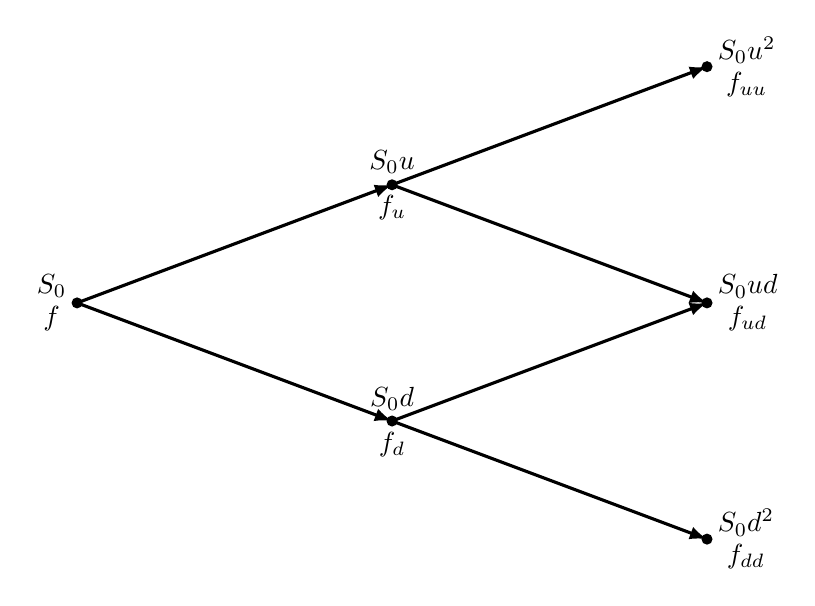
\begin{tikzpicture}[-latex, line width=0.4mm]
	\fill (0,0) circle (2pt) node [left] {\shortstack{\(S_0\) \\ \(f\)}};
	\fill (4,1.5) circle (2pt) node [above] {\(S_0u\)}
	node [below] {\(f_u\)};
	\fill (4,-1.5)  circle (2pt) node [above] {\(S_0d\)}
	node [below] {\(f_d\)};
	\fill (8,3) circle (2pt) 
	node [right] {\shortstack{\(S_0u ^ 2\) \\ \(f_{uu}\)}};
	\fill (8,0) circle (2pt) 
	node [right] {\shortstack{\(S_0ud\) \\ \(f_{ud}\)}};
	\fill (8,-3) circle (2pt) 
	node [right] {\shortstack{\(S_0d ^ 2\) \\ \(f_{dd}\)}};
	\draw (0,0) -- (4,1.5);
	\draw (0,0) -- (4,-1.5);
	\draw (4,1.5) -- (8,3);
	\draw (4,1.5) -- (8,0);
	\draw (4,-1.5) -- (8,0);
	\draw (4,-1.5) -- (8,-3);
\end{tikzpicture}

\end{document}
